\documentclass{article}
\usepackage{graphicx} % Required for inserting images
\usepackage[margin=0.5in]{geometry}
\usepackage{tikz}

\title{IMO 1999}
\author{Said Landaverde}
\date{2026}

\begin{document}

\maketitle

\section{Problem 1}

\noindent{\large\emph{Note.} \(S\) is a finite collection of at least three dots in the plane. A bisector divides something into two equal parts. A centroid is a specific kind of center: it is the average position of all the dots.} \\
\noindent{\large \\
   Let $O$ be the centroid of $S$, obtained by averaging the coordinates of its points. For any two distinct points $A,B\in S$,
   the perpendicular bisector of $AB$ passes through $O$. A reflection across this bisector maps \(S\) onto itself, so it fixes its centroid \(O\)
   and sends \(A\) to \(B\), so \(OA\) = \(OB\).

    \begin{center}
        \begin{picture}(120,50)
            \put(10,15){\line(1,0){100}}
            \multiput(60,10)(0,5){8}{\line(0,1){3}}
            \put(10,15){\line(5,2){50}}
            \put(110,15){\line(-5,2){50}}
            \put(7,3){$A$}
            \put(107,3){$B$}
            \put(60,35){\circle*{3}}
            \put(66,33){$O$}
            \put(10,15){\circle*{3}}
            \put(110,15){\circle*{3}}
            \put(33,30){\line(2,-5){4}}
            \put(83,20){\line(2,5){4}}
        \end{picture}
    \end{center}

    \noindent Thus all points of \(S\) lie on a circle centered at \(O\). Because \(A\) and \(B\) were arbitrary, every point has the same distance from \(O\). That shared distance is the circle's radius.
    \\\\
    Let \(P=A, Q, R=B\) be any three consecutive points of \(S\) in clockwise order. If you walk clockwise from \(P\) to \(R\), \(Q\) is the only dot you pass. This gives us two neighboring gaps to compare, one on each side of \(Q\).
    Reflect across the perpendicular bisector of \(PR\).
    This reflection maps the clockwise arc from \(P\) to \(R\) onto itself.

    \begin{center}
    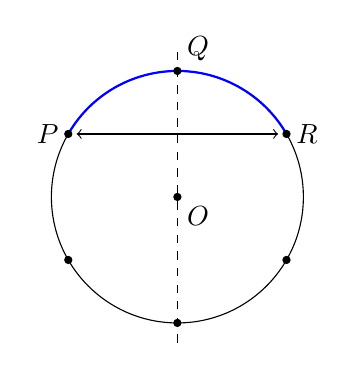
\begin{tikzpicture}
        \coordinate (P) at (150:1.6);
        \coordinate (Q) at (90:1.6);
        \coordinate (R) at (30:1.6);

        \draw (0,0) circle (1.6);
        \draw[blue, thick] (P) arc[start angle=150, end angle=30, radius=1.6];
        \draw[dashed] (0,-1.85) -- (0,1.85);
        \draw[<->, shorten <=3pt, shorten >=3pt] (P) -- (R);
        
        \fill (P) circle (1.5pt) node[left] {$P$};
        \fill (Q) circle (1.5pt) node[above right] {$Q$};
        \fill (R) circle (1.5pt) node[right] {$R$};
        \fill (0,0) circle (1.5pt) node[below right] {$O$};

        \foreach \angle in {210,270,330}
            \fill (\angle:1.6) circle (1.5pt);
    \end{tikzpicture}
    \end{center}

    Since \(Q\) is the only point of \(S\) inside this arc, the reflection fixes \(Q\).
}

\end{document}
